\section{Question 1}
System:
$$
G_{1_{(s)}} = \dfrac{1}{(s+1)(2s+1)}\exp(-s) = \dfrac{1}{2s^2+3s+1}
$$
We use Optimal PID to design controller with ITAE, ISE and IAE cont function.
\newpage
 \begin{itemize}
     \item ITAE
     $$
     K_p = 1.6922, \quad K_i = 0.5472, \quad K_d = 1.3675
     $$
     \begin{figure}[H]
        \caption{Step responde with PID controller and ITAE cost function}
        \centering
        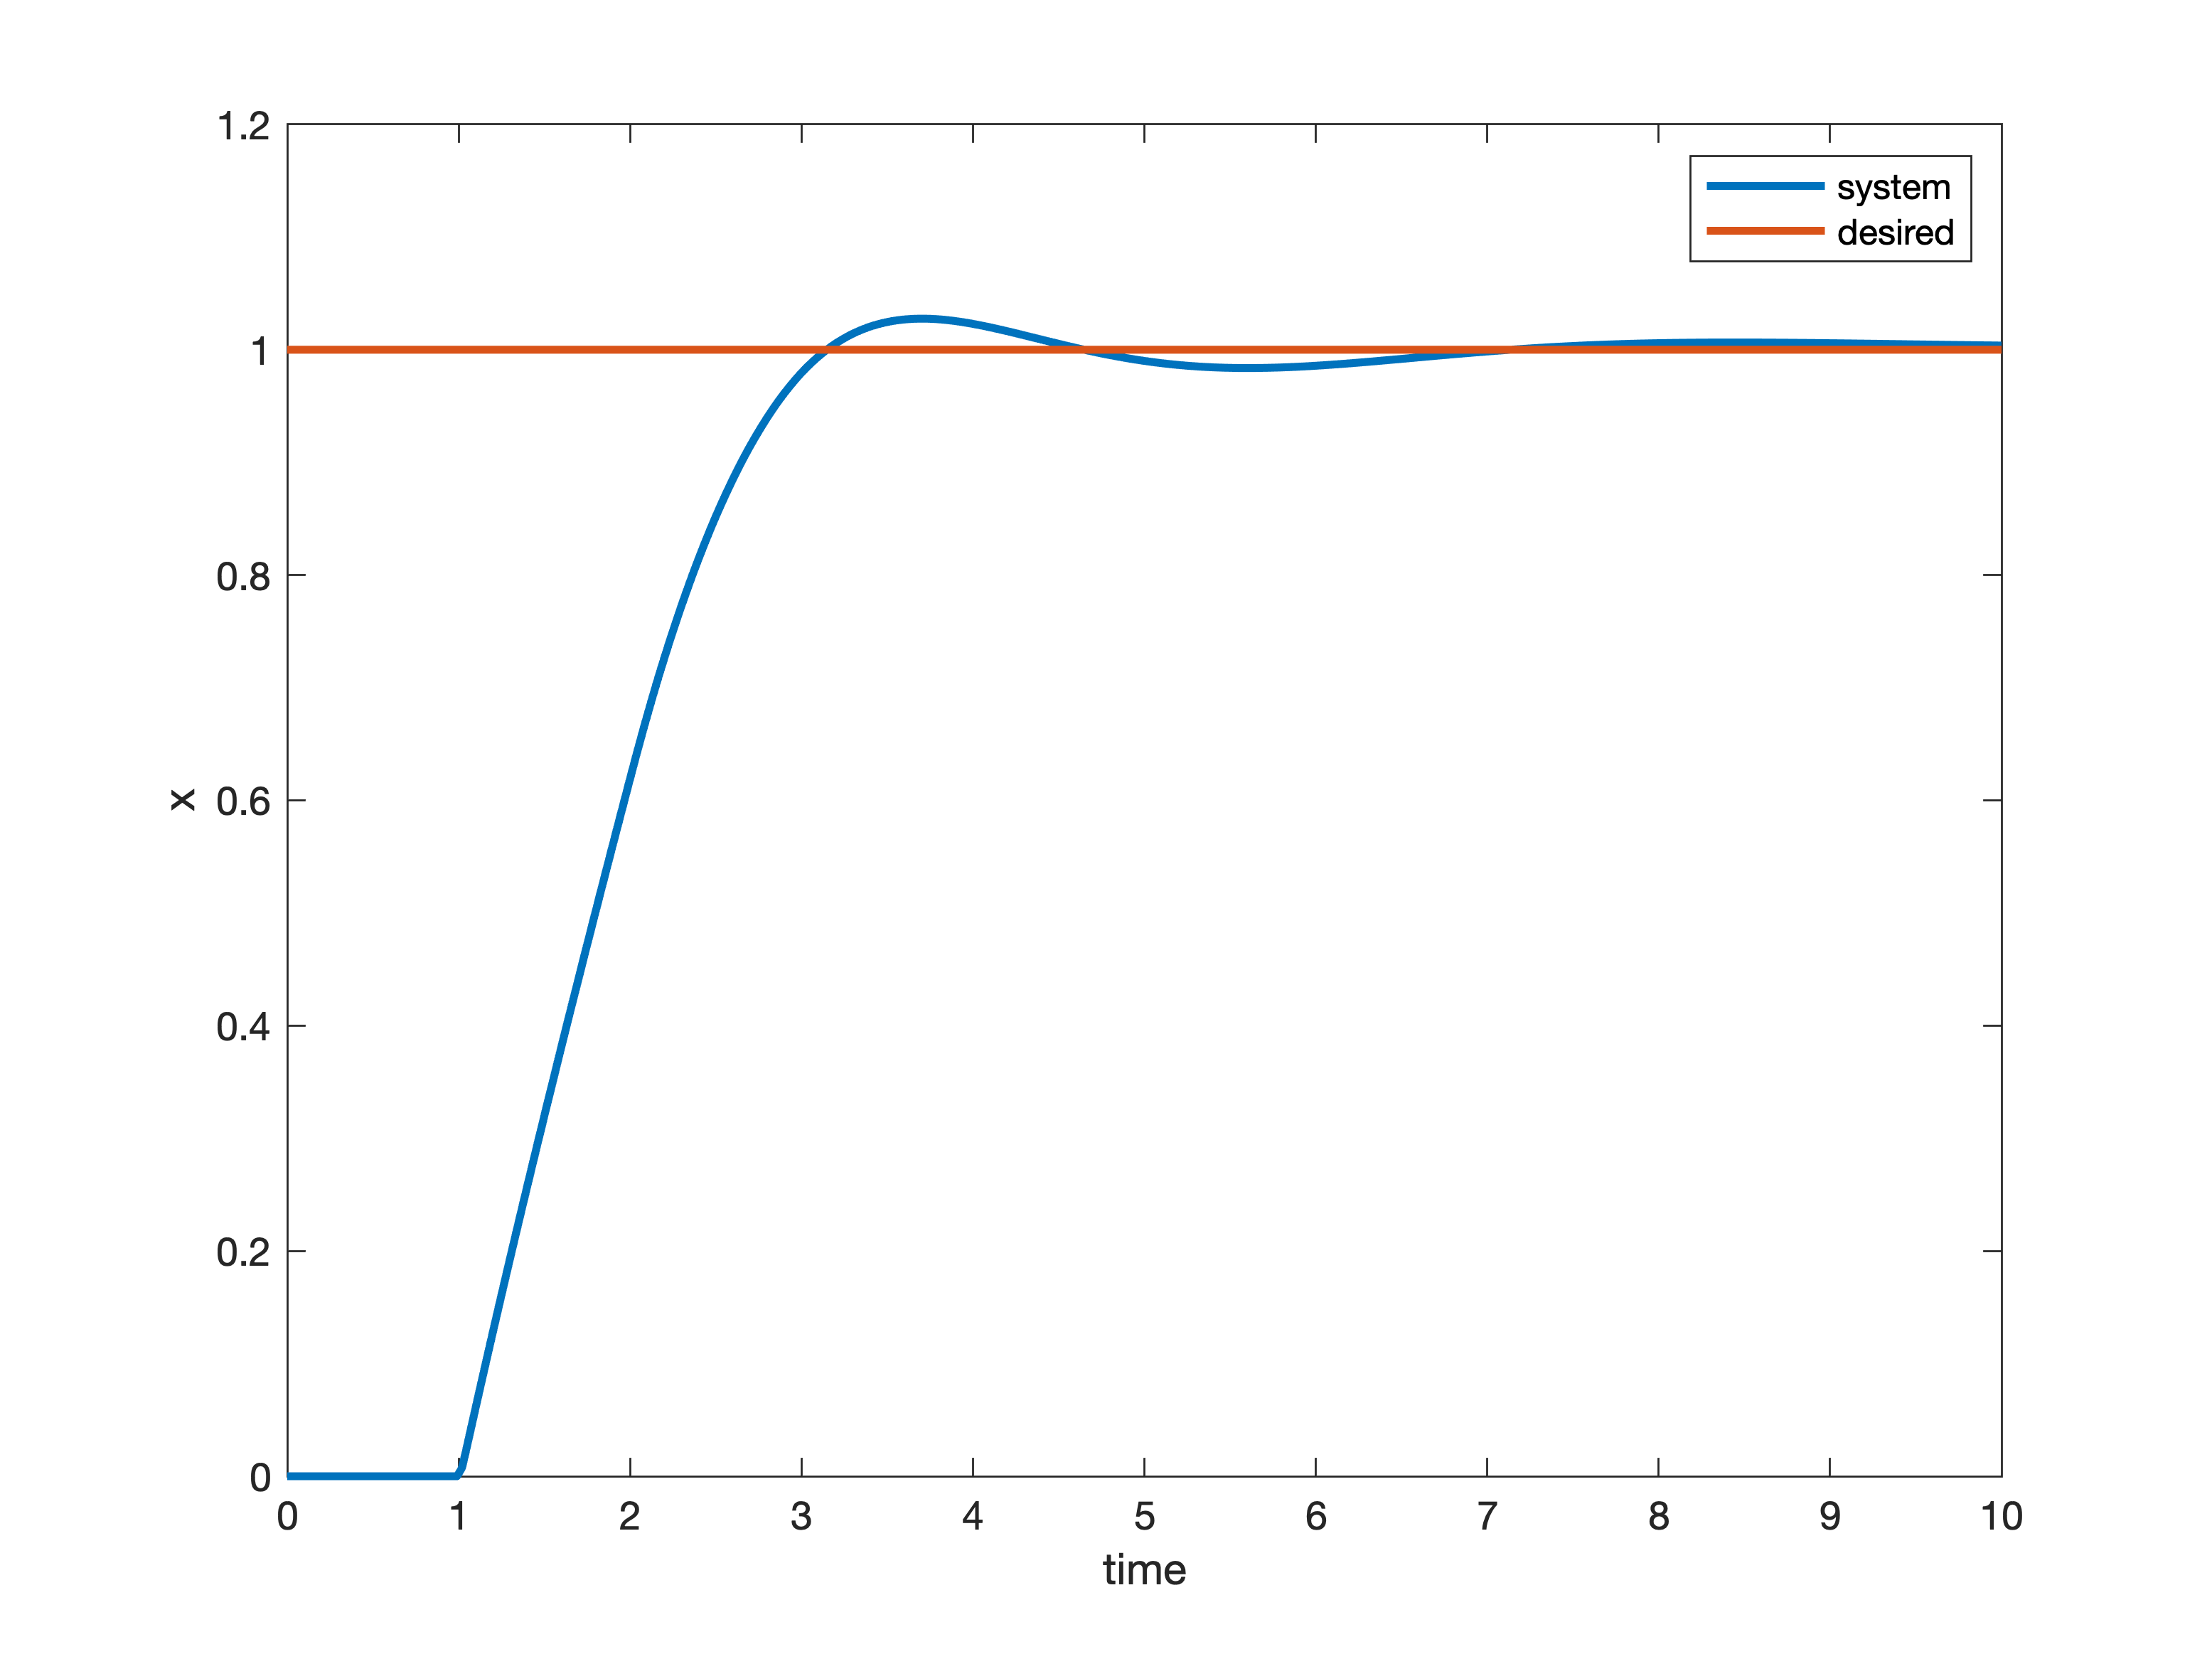
\includegraphics[width=11cm]{../Figure/Q1/ITAE.png}
    \end{figure}
    \item ISE
    $$
    K_p =1.8957, \quad K_i = 0.8007, \quad  K_d =2.5416
    $$
    \begin{figure}[H]
       \caption{Step responde with PID controller and ISE cost function}
       \centering
       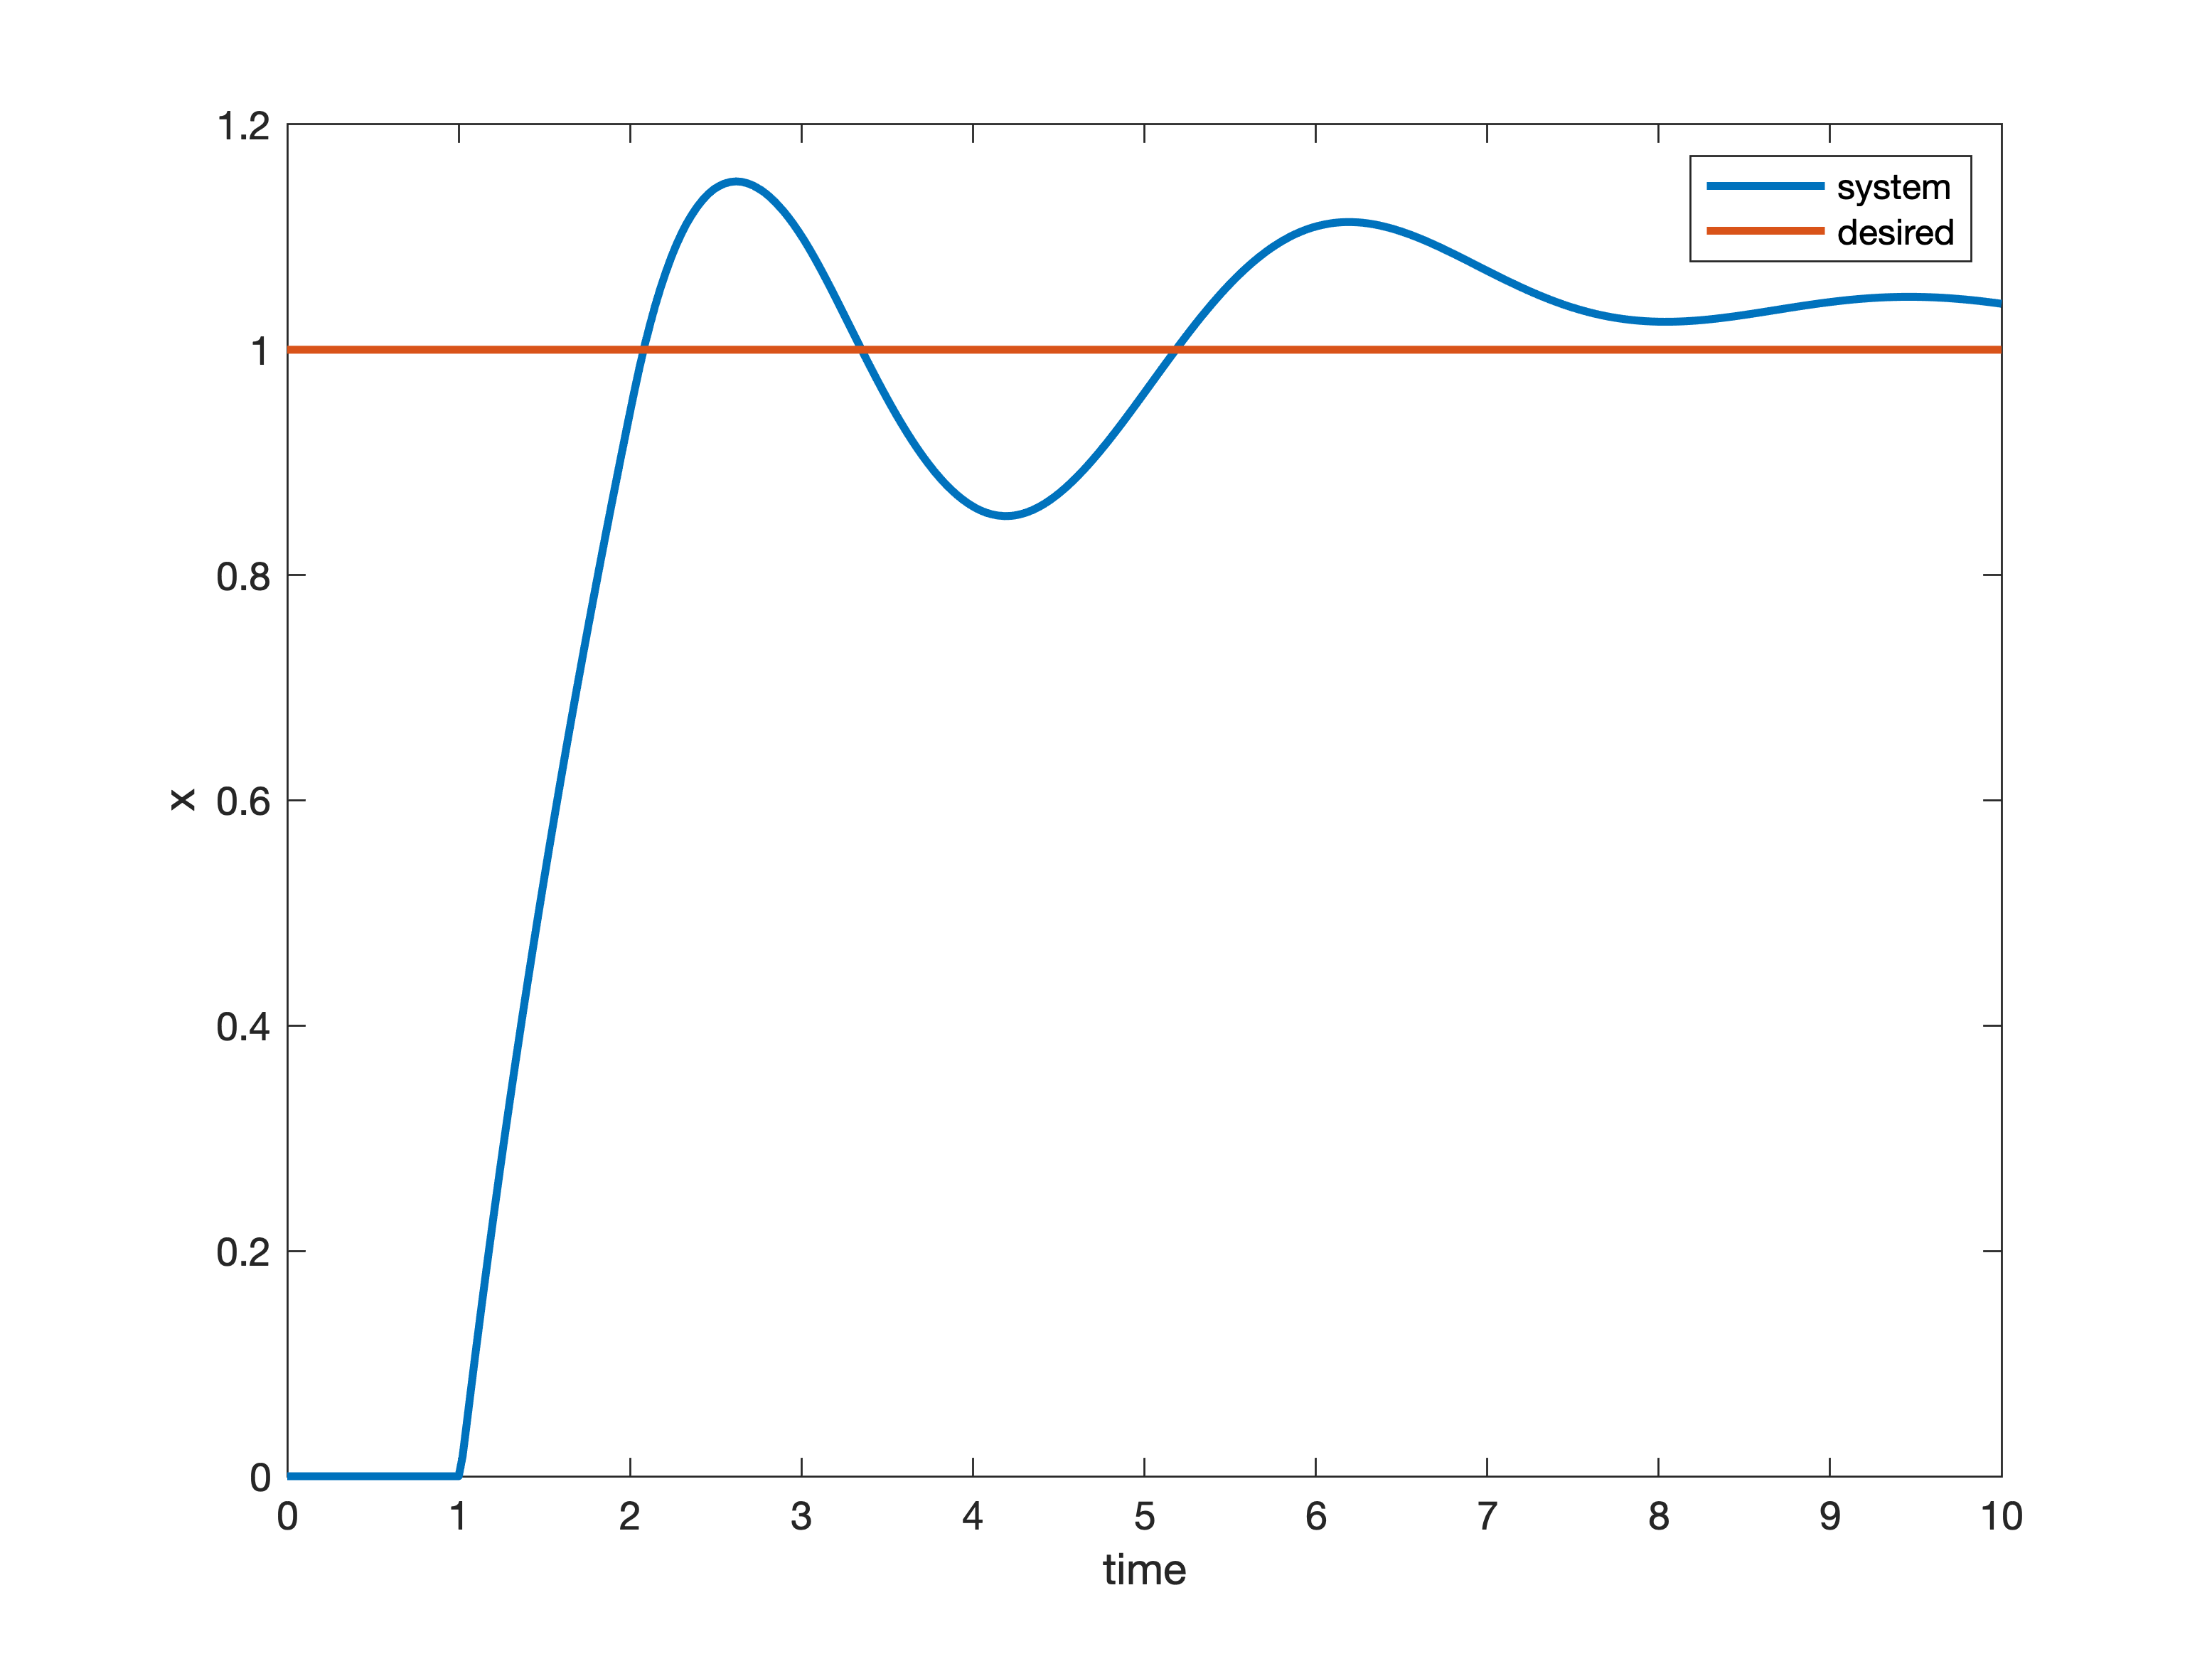
\includegraphics[width=11cm]{../Figure/Q1/ISE.png}
   \end{figure}
   \item IAE
   $$
   K_p = 1.8356, \quad K_i = 0.6085, \quad K_d = 1.7386
   $$
   \begin{figure}[H]
      \caption{Step responde with PID controller and IAE cost function}
      \centering
      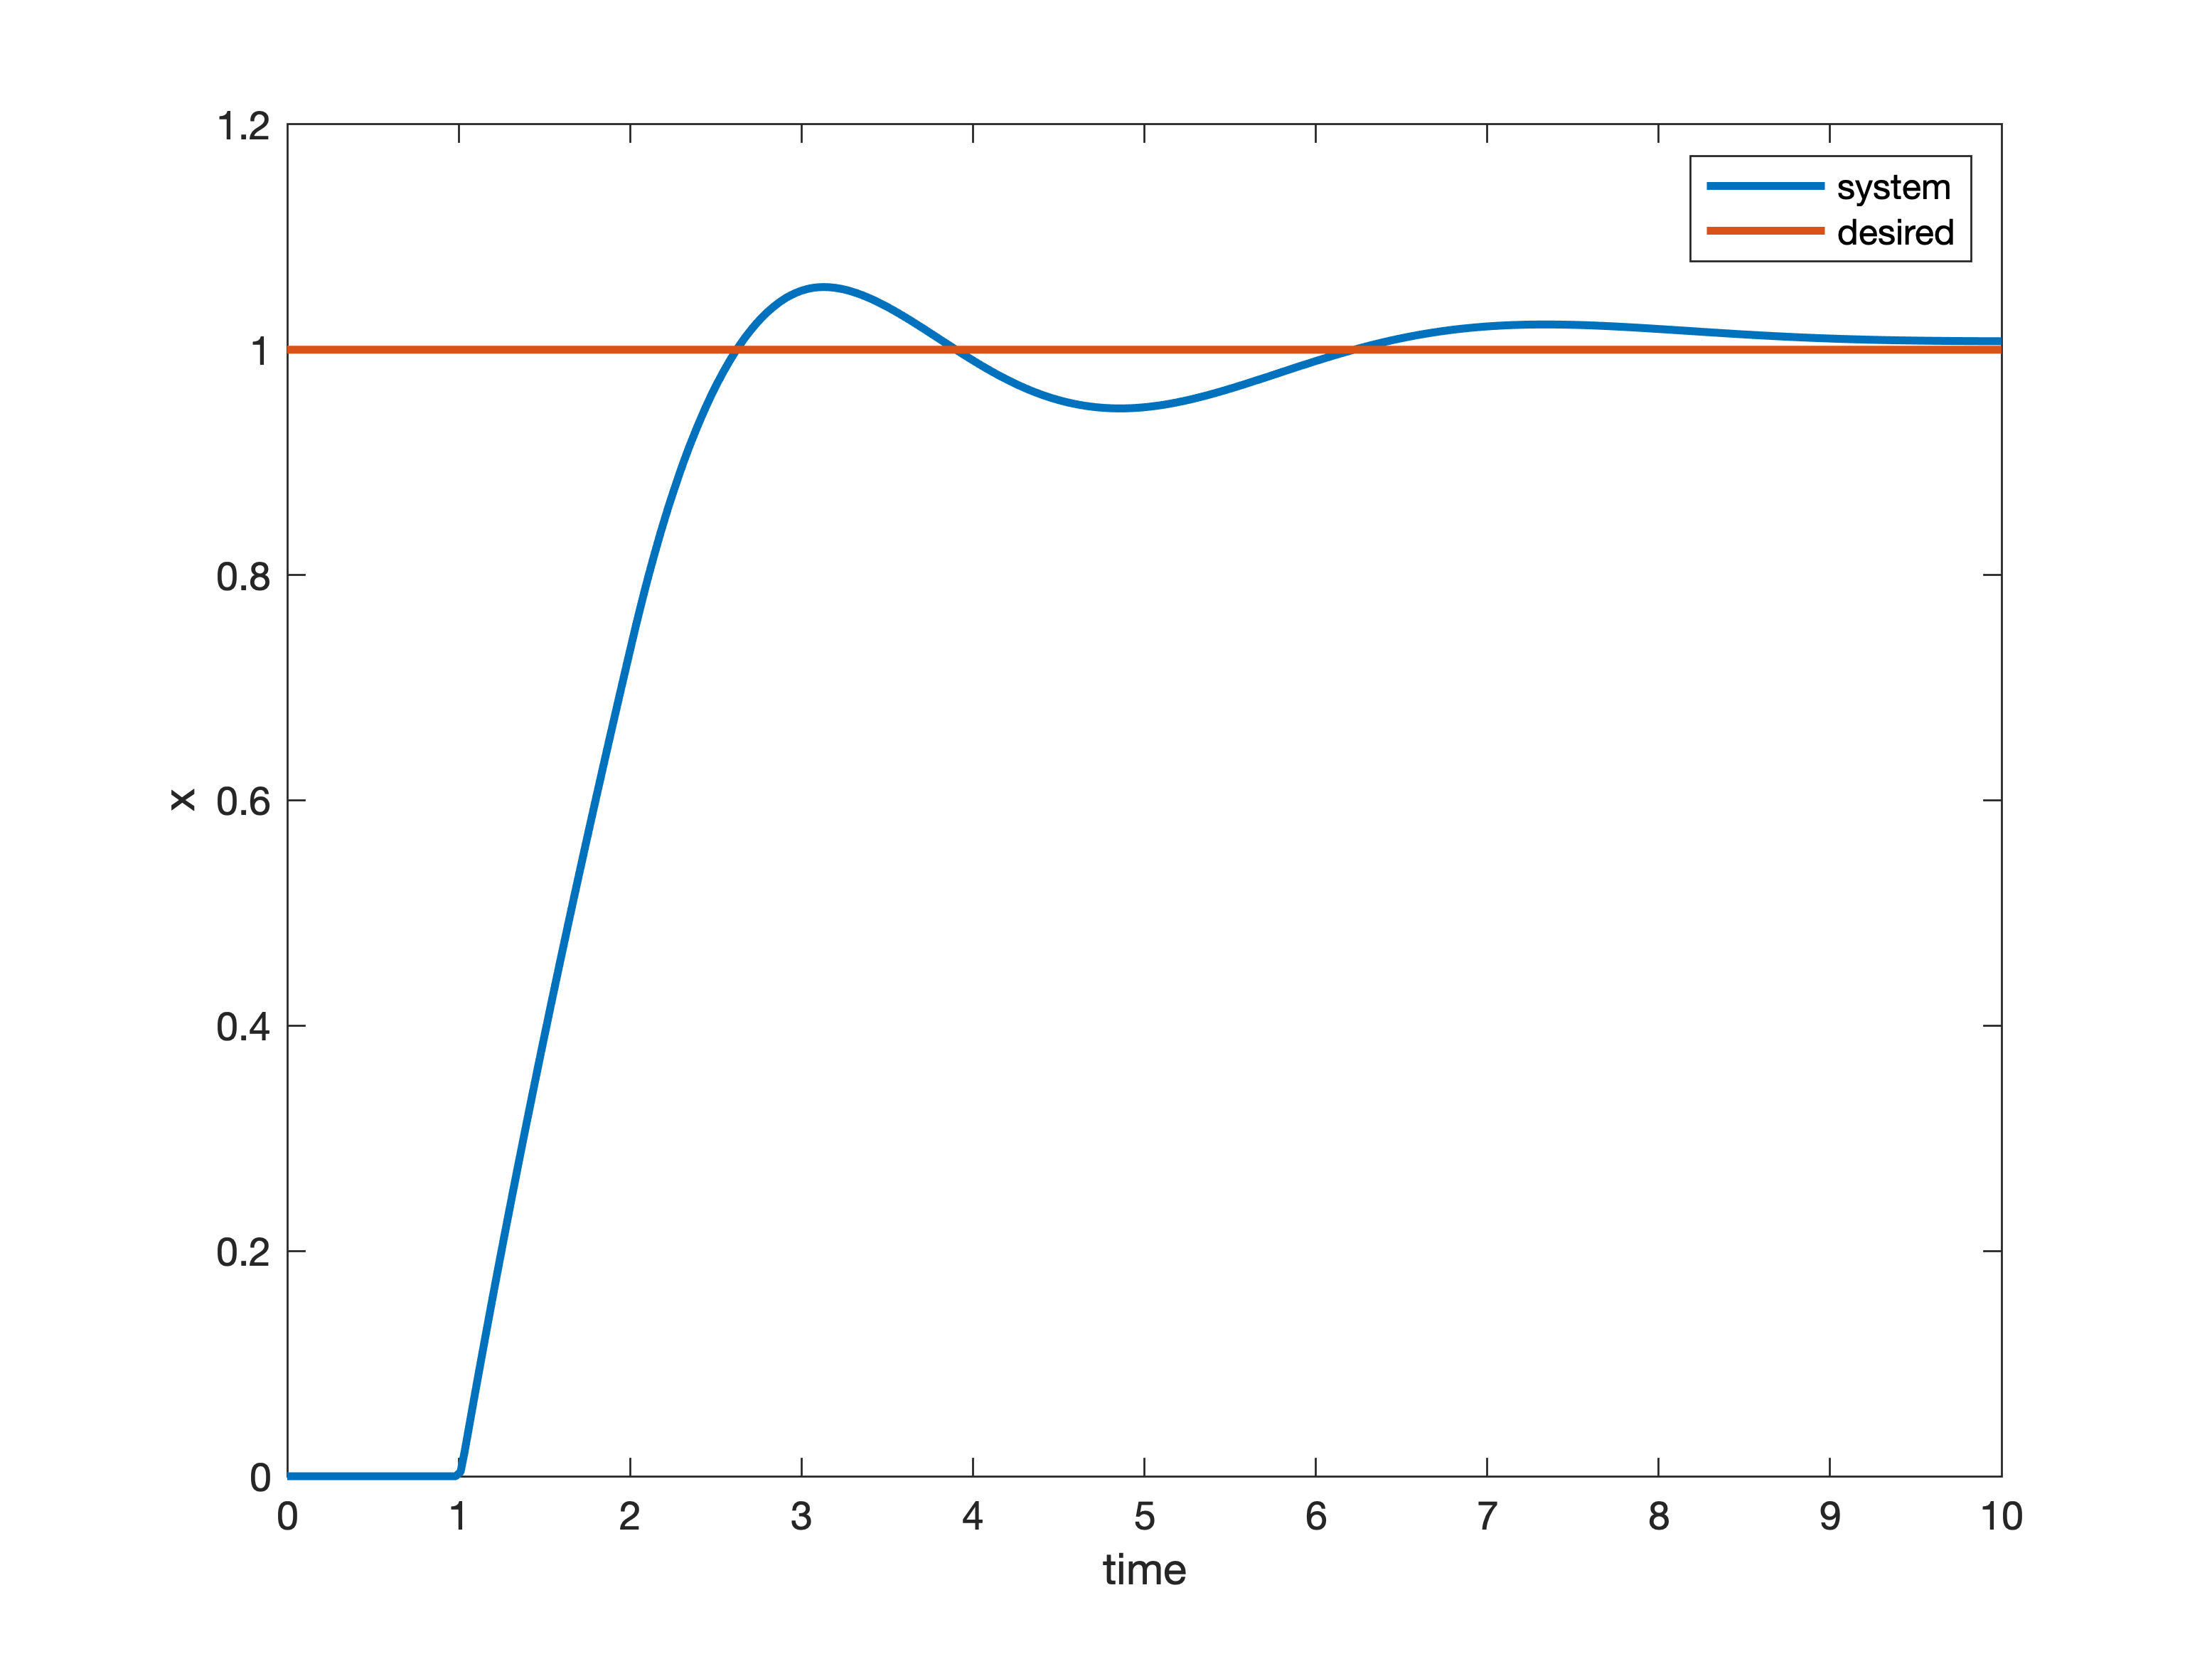
\includegraphics[width=11cm]{../Figure/Q1/IAE.png}
  \end{figure}
 \end{itemize}
 PID designed with ITAE cost function work better system is fast with lower overshoot.